% ---
% Capa
% ---
\imprimircapa
% ---

% ---
% Folha de rosto
% (o * indica que haverá a ficha bibliográfica)
% ---
\imprimirfolhaderosto*
% ---

% ---
% Inserir a ficha bibliografica
% ---
% http://ficha.bu.ufsc.br/
% \begin{fichacatalografica}
% 	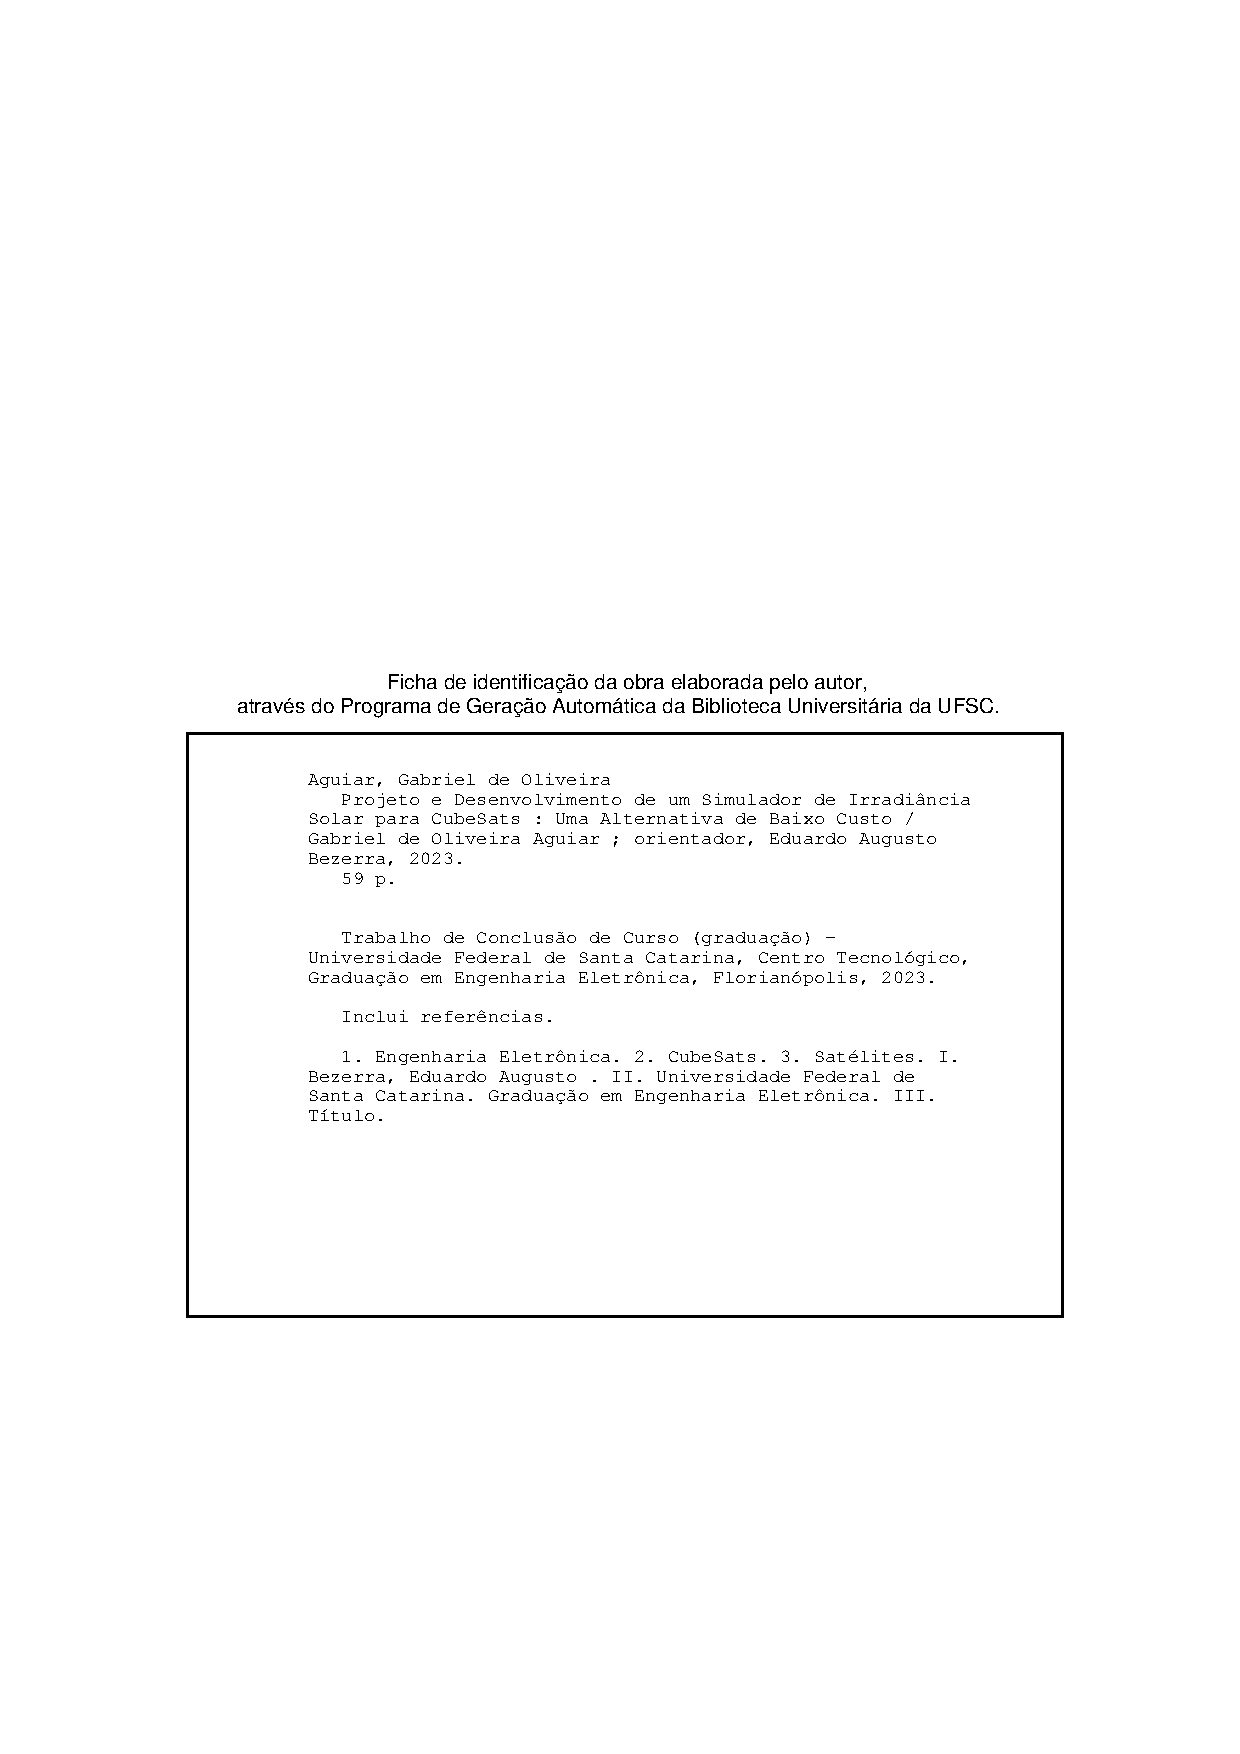
\includepdf{beforetext/Ficha_Catalografica.pdf}
% \end{fichacatalografica}
% ---

% ---
% Inserir folha de aprovação
% ---
% \begin{folhadeaprovacao}
% 	\OnehalfSpacing
% 	\centering
% 	\imprimirautor\\%
% 	\vspace*{10pt}		
% 	\textbf{\imprimirtitulo}%
% 	\ifnotempty{\imprimirsubtitulo}{:~\imprimirsubtitulo}\\%
% 	\vspace*{\baselineskip}
% 	This Master's Thesis was deemed suitable for the attainment of the Master of Science in Computer Science and was approved in its final form by the Graduate Program in Computer Science of INE - Department Of Informatics and Statistics, CTC - Technological Center of Universidade Federal de Santa Catarina.\\
%     \vspace*{\baselineskip}
%     Florianópolis, July 14, 2025. \\
% 	\vspace*{\baselineskip}
%  	\assinatura{\OnehalfSpacing Prof. xxxxxxx, Ph.D. \\ Graduate Program Coordinator}

%  	\vspace*{\baselineskip}
% 	\textbf{Examination Committee}\\
% 	\assinatura{\OnehalfSpacing\imprimirorientador \\ \imprimirorientadorRotulo}
% 	\vspace*{\fill}
%  	\assinatura{\OnehalfSpacing xxxxxxx, Eng.\\
% 	Federal University of Santa Catarina}
% 	\vspace*{\fill}
%  	\assinatura{\OnehalfSpacing xxxxxxx, M.Sc.\\
% 	Federal University of Santa Catarina\\}
% 	\vspace*{\fill}
% 	\assinatura{Prof. xxxxxxx, Ph.D.\\
% 	Federal University of Santa Catarina}

% 	\vspace*{\fill}
% 	\imprimirlocal, \imprimirano.
% \end{folhadeaprovacao}

% ---

% ---
% Dedicatória
% ---
% \begin{dedicatoria}
% 	\vspace*{\fill}
% 	\noindent
% 	\begin{adjustwidth*}{}{5.5cm} 
% 		\raggedleft       
% 		Sou grato aos meus amigos e familiares, que me apoiaram emocionalmente ao longo desta jornada acadêmica.
% 	\end{adjustwidth*}
% \end{dedicatoria}
% ---

% ---
% Agradecimentos
% ---
% \begin{agradecimentos}
% Aos meus amados pais, Leila Rosa de Oliveira e Antonio Neto Aguiar, que sempre estiveram ao meu lado, me apoiando incondicionalmente e estimulando minha busca pelo conhecimento.

% Ao meu dedicado orientador, Eduardo Bezerra, pelo seu valioso suporte, paciência e dedicação ao longo deste trabalho, além de disponibilizar o espaço no SPACELAB, que foi fundamental para a realização deste artigo.

% Agradeço de coração ao grupo AZCD, do qual faço parte e considero uma verdadeira família, pelo apoio inestimável. Sem eles, eu não seria quem sou hoje.

% Aos meus colegas do SPACELAB, em especial a João Cláudio Elsen Barcellos, pelo apoio direto no projeto e por incentivarem minhas ideias com entusiasmo.

% E, por fim, gostaria de expressar minha gratidão à Carolina Bassi, minha leal namorada e parceira, por seu apoio constante ao longo dessa jornada acadêmica.
% \end{agradecimentos}
% ---

% ---
% Epígrafe
% ---
% \begin{epigrafe}
% 	\vspace*{\fill}
% 	\begin{flushright}
% 		\textit{``The ideal engineer is a composite... \\ He is not a scientist, he is not a mathematician, \\he is not a sociologist or a writer;\\ but he may use the knowledge and techniques \\ of any or all of these disciplines in solving engineering problems.''\\
% 			(Dougherty, 1955)}
% 	\end{flushright}
% \end{epigrafe}
% ---

% ---
% RESUMOS
% ---

% resumo em português

\setlength{\absparsep}{18pt} % ajusta o espaçamento dos parágrafos do resumo
\begin{resumo}[Resumo]
	\SingleSpacing
	Alertas de colisão em comunicação veículo-a-tudo (\emph{Vehicle-to-Everything}, V2X) são mensagens raras, porém de alto impacto, cuja utilidade depende de entrega oportuna sob contenção de canal. Em redes IEEE 802.11p descentralizadas, esses alertas compartilham o meio com o tráfego de rotina, de modo que picos de atraso e congelamento de \emph{backoff} podem corroer sua prioridade sob carga. Esta dissertação avalia uma estratégia focada de priorização ciente de colisão na qual todos os veículos trocam tráfego \emph{multicast} periódico de melhor esforço (\emph{Best Effort}, BE), enquanto um veículo acidentado emite rajadas temporárias de alerta marcadas com \emph{Differentiated Services Code Point} (DSCP) 46 e mapeadas para a categoria de voz (\emph{Voice}, VO). Usando OMNeT++, Veins e INET, cinco políticas de controle de acesso ao meio (MAC) são comparadas em cenários de rodovia com 10 e 100 veículos: uma linha de base com \emph{Distributed Coordination Function} (DCF), \emph{Enhanced Distributed Channel Access} (EDCA) com mapeamento explícito de DSCP para voz, e três extensões adaptativas que temporariamente adiam ou descartam o tráfego BE concorrente enquanto os alertas estão ativos, todas sem exigir mudanças de protocolo ou infraestrutura. Sob congestionamento intenso, a preempção de emergência reduz o atraso de percentil 95 dos alertas de colisão em cerca de 49\% em relação ao EDCA (de 0,90 ms para 0,46 ms), ao custo de maior atraso BE e perdas BE explícitas; sob contenção leve, a supressão limitada penaliza principalmente o BE sem melhorar os alertas. Os resultados caracterizam uma fronteira proteção-custo e indicam que o bloqueio adaptativo deve ser uma escalada acionada por eventos, e não um modo de QoS permanentemente ativo.

	\textbf{Palavras-chave}: V2X. Wi-Fi Veicular. IEEE 802.11p. EDCA. Qualidade de Serviço. Priorização Ciente de Colisão.
\end{resumo}

% resumo em inglês
\begin{resumo}[Abstract]
	\SingleSpacing
	\begin{otherlanguage*}{english}
	Vehicle-to-everything (V2X) crash alerts are rare but high-impact messages whose usefulness depends on timely delivery under channel contention. In decentralized IEEE 802.11p networks they share the medium with routine traffic, so delay spikes and backoff freezing can erode their priority under load. This dissertation evaluates a focused crash-aware prioritization strategy in which all vehicles exchange periodic Best Effort (BE) multicast traffic while one crash vehicle emits temporary alert bursts marked with Differentiated Services Code Point (DSCP) 46 and mapped to Voice (VO). Using OMNeT++, Veins, and INET, five Medium Access Control (MAC) policies are compared on highway scenarios with 10 and 100 vehicles: a Distributed Coordination Function (DCF) baseline, Enhanced Distributed Channel Access (EDCA) with explicit DSCP-to-Voice mapping, and three adaptive extensions that temporarily suppress or drop competing BE traffic while alerts are active, all requiring no protocol changes or infrastructure. Under heavy congestion, emergency preemption reduces crash-alert 95th-percentile delay by about 49\% relative to EDCA (from 0.90 ms to 0.46 ms), at the cost of higher BE delay and explicit BE losses; under light contention, bounded suppression mainly penalizes BE without improving alerts. The results characterize a protection-versus-cost frontier and indicate that adaptive blocking should be an event-triggered escalation rather than an always-on QoS mode.

		\textbf{Keywords}: V2X. Vehicular Wi-Fi. IEEE 802.11p. EDCA. Quality of Service. Crash-Aware Prioritization.
	\end{otherlanguage*}
\end{resumo}

%% resumo em francês 
%\begin{resumo}[Résumé]
% \begin{otherlanguage*}{french}
%    Il s'agit d'un résumé en français.
% 
%   \textbf{Mots-clés}: latex. abntex. publication de textes.
% \end{otherlanguage*}
%\end{resumo}
%
%% resumo em espanhol
%\begin{resumo}[Resumen]
% \begin{otherlanguage*}{spanish}
%   Este es el resumen en español.
%  
%   \textbf{Palabras clave}: latex. abntex. publicación de textos.
% \end{otherlanguage*}
%\end{resumo}
%% ---

{%hidelinks
	\hypersetup{hidelinks}
	% ---
	% inserir lista de ilustrações
	% ---
	\pdfbookmark[0]{\listfigurename}{lof}
	\listoffigures*
	\cleardoublepage
	% ---
	
	% ---
	% inserir lista de quadros
	% ---
	% \pdfbookmark[0]{\listofquadrosname}{loq}
	% \listofquadros*
	% \cleardoublepage
	% ---
	
	% ---
	% inserir lista de tabelas
	% ---
	\pdfbookmark[0]{\listtablename}{lot}
	\listoftables*
	\cleardoublepage
	% ---
	
	% ---
	% inserir lista de abreviaturas e siglas (devem ser declarados no preambulo)
	% ---
	% \imprimirlistadesiglas
	% ---
	
	% ---
	% inserir lista de símbolos (devem ser declarados no preambulo)
	% ---
	% \imprimirlistadesimbolos
	% ---
	
	% ---
	% inserir o sumario
	% ---
	\pdfbookmark[0]{\contentsname}{toc}
	\tableofcontents*
	\cleardoublepage
	
}%hidelinks
% ---